\documentclass{article}
\usepackage{blindtext}
\usepackage[utf8]{inputenc}
\usepackage{amsmath,bm}
\usepackage{amstext}
\usepackage{amsfonts}
\usepackage{amsmath}
\usepackage{epsfig}
\usepackage[UTF8]{ctex}
\usepackage[colorlinks,linkcolor=blue]{hyperref}

\title{Introduction to Machine Learning\\Homework 3}
\author{吴紫航 171860659}
\date{} 
\begin{document}
	\maketitle
	\numberwithin{equation}{section}
	
	\section{[20pts] Decision Tree}

	(1) [10pts] Assume there is a space contains three binary features $X$, $Y$, $Z$ and the objective function is $f(x,y,z)=\neg(x \text{ XOR } y)$. Let $H$ denotes the decision tree constructed by these three features. Please answer the following question:
	\begin{itemize}
		\item Is function $f$ realizable? 
		\\答:函数可实现为决策树
		\item If the answer is yes, please draw the decision tree $H$ otherwise please give the reason.\\
		答:决策树见下图
		\begin{figure}[htbp]
			\centering
			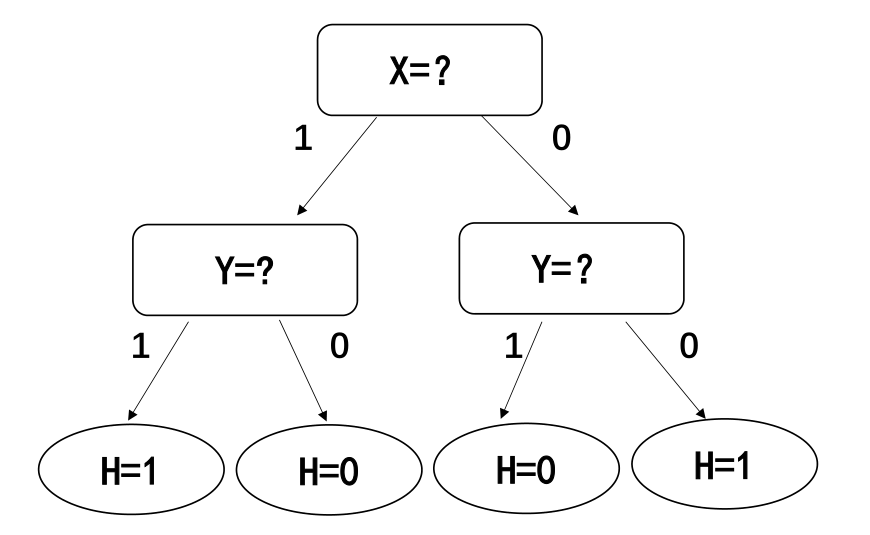
\includegraphics[scale=0.5]{decisionTree_1_1.png}
			\caption{decision tree of H}
		\end{figure}
	\end{itemize}
	
	

	(2) [20pts] Consider the following matrix:
	$$
	\left[
	\begin{matrix}
	24 & 53 & 23 & 25 & 32 & 52 & 22 & 43 & 52 & 48 \\
	40 & 52 & 25 & 77 & 48 & 110 & 38 & 44 & 27 & 65\\
	\end{matrix}
	\right]
	$$
	which contains 10 examples and each example contains two features $x_1$ and $x_2$. The corresponding label of these 10 examples as follows:
	$$
	\left[
	\begin{matrix}
	1 & 0 & 0 &1 & 1 & 1 & 1& 0 & 0 & 1
	\end{matrix}
	\right]
	$$
	In this problem, we want to build a decision tree to do the classification task.
	\begin{itemize}
		\item Calculate the entropy of the root node.
		\\解:总的信息熵$E_{root}=-0.6log_{2}0.6-0.4log_{2}0.4=0.97095$
		\item Building your decision tree. What is your split rule  and the classification error?\\
		解:对于连续属性,我们可以用二分类的方法转换为离散属性。具体的来说,使用信息增益的方法进行划分,由于划分前的信息熵$E_{root}$相同,因此只要找到划分后条件信息熵最小的情况即可。
		\\对于第一行属性,经过计算,使用52作为分隔点时,条件熵最小:\\$E_{minCondtion1}=0.9\times[\frac{3}{9}log(\frac{9}{3})+\frac{6}{9}log(\frac{9}{6})]+0.1\times[1log(1)+0log(0)]$\\$=0.826466$\\
	对于第二行属性,经过计算,使用27作为分隔点时,条件熵最小:\\$E_{minCondtion2}=0.2\times[1log(1)+0log(0)]+0.8\times[\frac{1}{4}log(\frac{4}{1})+\frac{3}{4}log(\frac{4}{3})]$\\$=0.64902$\\
	因此第一层划分判断为: $x_2\leq 27?$\\
	划分后,忽略第二行属性并加上$\bm{label}$值进行增广,得到下面两个矩阵
	$$
	M_1=\left[
	\begin{matrix}
	24 & 53 & 25 & 32 & 52 & 22 & 43 & 48\\
	1 & 0 & 1 & 1 & 1 & 1 & 0 & 1 \\
	\end{matrix}
	\right]
	$$
	$$
	M_2=\left[
	\begin{matrix}
	23 & 52\\
	0 & 0\\
	\end{matrix}
	\right]
	$$
	\\我们发现$M_2$已经可以确定分类结果为$0$,那么只需要再用信息增益最大化的方法,对$M_1$的分隔点进行运算,得到:
	\\$M_1$的分隔点为32,条件熵为$0.5$,故子分枝判断条件为 $x_1\leq 32?$
\\本题采用的划分方法是信息增益法
	\\确定的决策树如下图。
\\错误分类的样本有:
\\第$6$列:“$x1=52,x2=110$”,其真实的label为$1$,但决策树预测为$0$;
\\第$10$列:“$x1=48,x2=65$”,其真实的label为$1$,但决策树预测为$0$;
	\begin{figure}[htbp]		
			\centering
			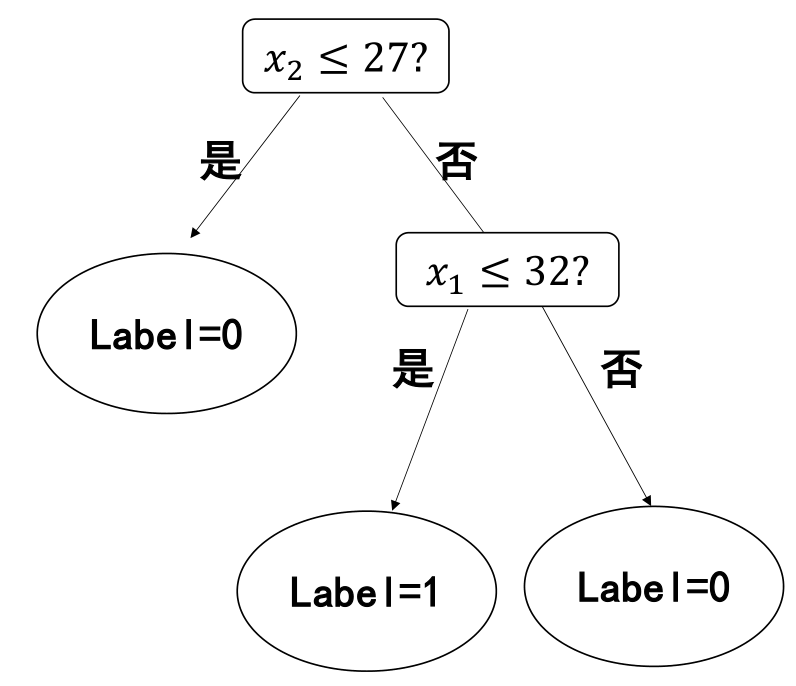
\includegraphics[scale=0.5]{decisionTree_1_2.png}
			\caption{decision tree of label}
		\end{figure}
	\end{itemize}

	\section{[20pts] Neural Network}
	Consider the following neural network, consisting of two input units, a single hidden layer containing two units, and one output unit:
	
	\begin{figure}[htbp]
		\centering
		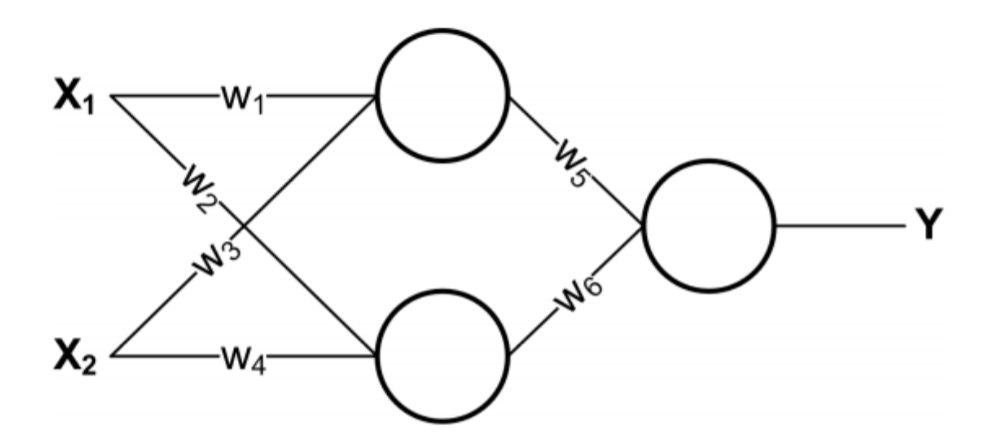
\includegraphics[scale=0.5]{figure_nn.png}
		\caption{Neural network structure for problem 3.}
	\end{figure}

	(1) [5pts] Assume that the network is using linear units: that is, for a given unit $U$, $A$ is the vector of activations of units that send their output to $U$ and $W$ is the weight vector corresponding to these outputs, then the output of the unit is $W^{\top}A$ Let the weight values $w_i$ be fixed, re-design the neural network to compute the same function without using any hidden units. Express the new weights in terms of the old weights.

	(2) [5pts] Is it always possible to express a neural network made up of only linear units without a hidden layer?\\
	
	(3) [10pts] Choose an activation function for each unit in the network which will cause this network to learn the same function that logistic regression would learn. each unit should use a logistic, linear, or threshold activation function, with no constraints on the weights.\\\\
	1) 解:
		由原图,隐藏层两个节点的输出为$w_1x_1+w_3x_2$和$w_2x_1+w_4x_2$\\
		因此,最终输出为$w_5(w_1x_1+w_3x_2)+w_6(w_2x_1+w_4x_2)$\\
		即$(w_1w_5+w_2w_6)x_1+(w_3w_5+w_4w_6)x_2$, 图结构如下:\\
		\begin{figure}[htbp]
			\centering
			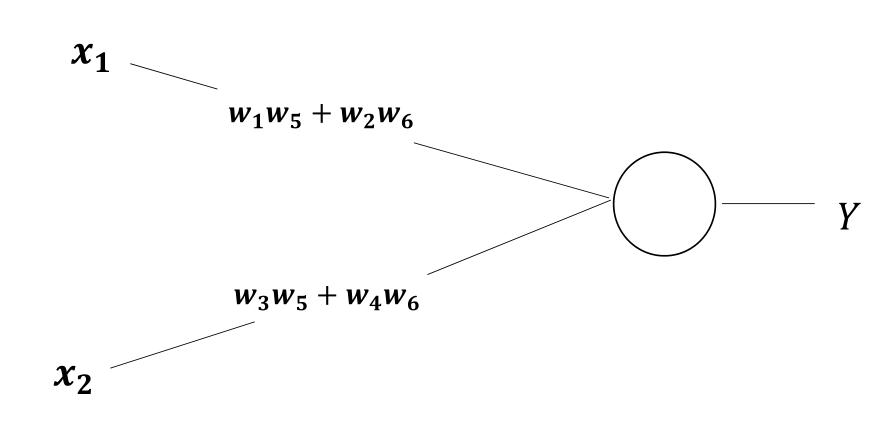
\includegraphics[scale=0.5]{NeuralNetwork_2_1.png}
			\caption{Equivalent neural network without hidden units}
		\end{figure}
	\\
	2) 解:
		对于没有隐层、且只有线性单元的神经网络,只能解决线性可分问题。例如异或这类非线性可分问题,学习过程将会来回震荡,无法收敛。\\
	\\3) 解:\\
	分析:\\Logistic regression可以看作隐层只有一个节点的神经网络,该节点的激活函数为sigmod函数。输出层激活函数是一个阶跃函数,即大于0就会通过阶跃函数激活,否则输出不激活。从而实现二分类。\\\\
	方法:\\由此,对于题目给定的神经网络结构(图3),我们将隐层的一个节点的激活函数设置为sigmod函数(即logistic function),隐层另一个节点的激活函数为置零函数(始终取常数0,显然属于linear function)。输出层的输出节点的激活函数为阶跃函数(threshold function)\\\\
	对比:\\这样的神经网络和Logistic Regression的效果是一样的:\\
	1)输入到隐层第一个节点的权重参数$w_1$、$w_2$和该隐层节点的阈值参数$\theta$对应于线性回归的参数$w_1$、$w_2$和$b$ ($b$与$\theta$互为相反数,效果都是bias偏置作用)。\\
	2)隐层第一个节点的激活函数sigmod函数对应于LR算法的sigmod函数\\
	3)隐层第二个节点被置零函数忽略了(始终不激活)\\
	4)隐层第一个节点到输出节点的权重参数$w_5$和输出节点的阈值参数$\theta_{out}$对应于对数几率回归最终的阈值分类过程
	\\
	\section{[60 pts] Neural Network in Practice}
	
	In this task, you are asked to build a Convolutional Neural Networks (CNNs) from scratch and examine performance of the network you just build on \textbf{MNIST} dataset.
	Fortunately, there are some out-of-the-box deep learning tools that can help you get started very quickly. For this task, we would like to ask you to work with the \textbf{Pytorch} deep learning framework. Additionally, Pytorch comes with a built-in dataset class for MNIST digit classification task in the \textbf{torchvision} package, including a training set and a validation set. You may find a pytorch introduction at \href{https://pytorch.org/tutorials/beginner/blitz/cifar10_tutorial.html}{here}. Note that, you can use CPU or GPU for training at your choice.
	
	Please find the detailed requirements below.
	
	\begin{enumerate}
		    \item[(1)] [5 pts] You are encouraged to implement the code using \emph{Python3}, implementations in any other programming language will not be judged. Please name the source file (which contains the main function) as \emph{CNN\underline{\hspace{0.5em}}main.py}. Finally, your code needs to print the performance on the provided validation set once executed.
\\\\答:执行完CNN\_main.py代码,将打印训练过程和测试性能结果,如下图\\
		\begin{figure}[htbp]
			\centering
			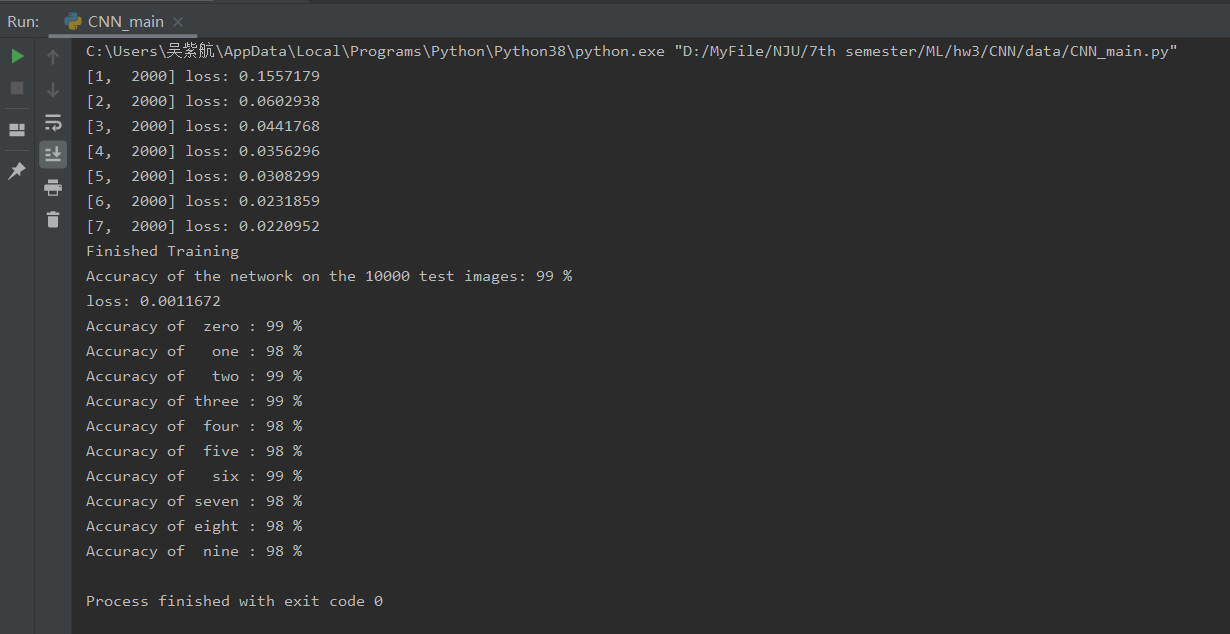
\includegraphics[scale=0.5]{Output_3_1.png}
			\caption{Output of Code CNN\_main.py}
		\end{figure}

		    \item[(2)] [10 pts] Use any type of CNNs as you want and draw graphs to show your network architecture in the submitted report. You are encouraged to try more architectures.
\\\\答:本题采用的神经网络结构如下图\\
		\begin{figure}[htbp]
			\centering
			\includegraphics[scale=0.5]{Architecture_3_2.png}
			\caption{Nerual Network Architecture}
		\end{figure}
		    
		    \item [(3)] [15 pts] During training, you may want to try some different optimization algorithms, such as SGD, Adam. Also, you need to study the effect of learning rate and the number of epoch, on the performance (accuracy).
 \\\\答:训练轮次epoch=7,每批次数目Batch size=30,SGD的学习速率lr=0.0001,动量momentum=0.9。此参数下测试总准确率accuracy为99\%\\
		    \item [(4)] [10 pts] Plot graphs (learning curves) to demonstrate the change of training loss as well as the validation loss during training.
\\答:loss曲线和前几问的具体细节写在报告report.pdf里\\
\end{enumerate}
\end{document}
